\documentclass[11pt]{article}
\usepackage[margin=1in]{geometry}
\usepackage{amsmath,amssymb}
\usepackage{booktabs}
\usepackage{graphicx}
\usepackage{adjustbox}
\usepackage{url}
\usepackage[T1]{fontenc}

\title{Revision Insert for SHIFT-ATCP Manuscript}
\author{}
\date{}

\begin{document}
\maketitle

\section*{Purpose}
This file contains the manuscript-level additions and replacements that should be merged into the main IEEE Access manuscript. It is based on the updated result folder \texttt{outputs\_dp\_shift\_atcp\_clinical\_novelty}. The goal is to make the paper clearer, reviewer-safe, and reproducible without rewriting the whole manuscript.

\section{Preamble Change}
For IEEE Access, avoid changing the default font family unless the journal specifically asks for it. In the old manuscript, remove or comment:
\begin{verbatim}
\usepackage[scaled]{helvet}
\renewcommand{\familydefault}{\sfdefault}
\end{verbatim}
Keep:
\begin{verbatim}
\usepackage[T1]{fontenc}
\end{verbatim}

\section{Title Replacement}
Replace the current title with the cleaner version below:
\begin{verbatim}
\title{SHIFT-ATCP: Shift-Aware and Diabetes-Protected Conformal Prediction
for Reliable Diabetes Classification Under Dataset Shift}
\end{verbatim}

\section{Shorter Abstract Replacement}
\begin{abstract}
Machine learning models for diabetes prediction may perform well in a source dataset but become unreliable when transported to a new clinical population. This study evaluates external diabetes model transportability from the Kaggle Diabetes Prediction Dataset to NHANES 2017--2018 and the Pima Indians Diabetes dataset. Five model families and three feature sets were evaluated under a leakage-safe protocol using fixed source, target-calibration, and target-test splits. To address external dataset shift, we introduce SHIFT-ATCP, a shift-aware conformal framework that estimates source trust using Population Stability Index, domain-classifier AUC, target calibration size, and prevalence shift. We further introduce DP-SHIFT-ATCP, a diabetes-protected variant that improves diabetes-positive class coverage using class-specific conformal thresholds. External shift was severe, with mean PSI values of 1.545 for NHANES and 1.897 for Pima and domain-classifier AUC of 1.000 for both target datasets. Conventional unweighted ATCP undercovered both targets, with mean 90\% coverage of 0.8468 on NHANES and 0.7612 on Pima. Safety-gated SHIFT-ATCP restored near-nominal marginal coverage, reaching 0.9031 on NHANES and 0.9059 on Pima. DP-SHIFT-ATCP improved diabetes-positive coverage from 0.6612 to 0.9090 on NHANES and from 0.8092 to 0.9280 on Pima, with larger prediction sets and referral rates. These results show that reliable external diabetes prediction requires not only discrimination and calibration but also shift-aware conformal uncertainty and class-wise clinical safety analysis.
\end{abstract}

\section{Contribution List Replacement}
Replace the current contribution list with:
\begin{itemize}
    \item We present a leakage-safe external diabetes transportability protocol with fixed source, target-calibration, and target-test partitions.
    \item We quantify source-target shift using PSI, domain-classifier AUC, prevalence shift, and source-trust estimation.
    \item We propose SHIFT-ATCP, a shift-aware target-dominant conformal method that automatically down-weights source calibration when source-target shift is severe.
    \item We propose DP-SHIFT-ATCP, a diabetes-protected conformal variant that improves diabetes-positive class coverage using class-specific thresholds.
    \item We report clinical reliability using marginal coverage, class-wise coverage, prediction-set size, referral rate, clinical cost, bootstrap confidence intervals, and target calibration-size ablation.
\end{itemize}

\section{Split Construction Paragraph to Add}
Add this paragraph after the split construction table:

For calibration method selection, the target calibration partition was further divided into target-calibration-fit and target-calibration-select subsets. The fit subset was used to fit the calibration model, whereas the select subset was used to choose the calibration method or conformal operating point. The target-test partition remained untouched until final evaluation. This design avoids target-test leakage and ensures that all final external results are reported only on held-out target-test data.

\section{ECE Split Table to Add}
\begin{table*}[!t]
\centering
\caption{Split-specific ECE reporting used in the revised leakage-safe protocol.}
\label{tab:ece_splits}
\begin{tabular}{lll}
\toprule
Evaluation purpose & Split used & Reported in \\
\midrule
Internal source performance & Kaggle internal test & Source-test and tuning results \\
Source calibration selection & Source calibration-select split & Calibration selection table \\
Adaptive target calibration selection & Target calibration-select split & Target calibration selection table \\
Final external performance & Held-out target-test split & External performance and clinical reliability tables \\
Bootstrap coverage intervals & Held-out target-test split & Bootstrap interval results \\
\bottomrule
\end{tabular}
\end{table*}

\section{PSI and Source-Trust Clarification}
Use the following table caption for the dataset shift table:

\begin{quote}
\textbf{Dataset shift metrics and shift-aware source trust.} PSI was computed using source-quantile bins, and domain AUC was computed by training a classifier to distinguish source from target records.
\end{quote}

\begin{table*}[!t]
\centering
\caption{Dataset shift metrics and shift-aware source trust. PSI was computed using source-quantile bins, and domain AUC was computed by training a classifier to distinguish source from target records.}
\label{tab:source_trust_insert}
\begin{tabular}{llrrrr}
\toprule
Target & Feature set & Mean PSI & Domain AUC & Prevalence gap & Source weight \\
\midrule
NHANES & Screening & 1.227 & 1.000 & 0.087 & 0.000476 \\
NHANES & Routine clinical & 1.545 & 1.000 & 0.087 & 0.000252 \\
NHANES & Extended transport & 1.545 & 1.000 & 0.087 & 0.000252 \\
Pima & Screening & 1.861 & 1.000 & 0.261 & 0.000164 \\
Pima & Routine clinical & 1.897 & 1.000 & 0.261 & 0.000152 \\
Pima & Extended transport & 1.897 & 1.000 & 0.261 & 0.000152 \\
\bottomrule
\end{tabular}
\end{table*}

\section{Hyperparameter Selection Rule to Add}
Add this paragraph in the model training subsection:

For each model family, three candidate settings were evaluated under the same source-validation budget. The selected setting was chosen using validation ROC-AUC as the primary criterion, followed by Brier score and ECE as secondary criteria. No target-test data were used for hyperparameter tuning.

\section{Weighted SHIFT-ATCP Explanation to Add}
Add this after the source-trust equation:

The weighted conformal threshold was computed from the combined source and target calibration nonconformity scores. Source calibration scores received weight $w_s$, whereas target calibration scores received weight 1.0. Therefore, when measured shift was severe, the source contribution became very small and the threshold became target-dominant. When source and target were more similar, source calibration could contribute more strongly.

\section{Clinical Cost Formula to Add}
The code used false-negative cost $c_{FN}=5.0$, false-positive cost $c_{FP}=1.0$, uncertain/referral cost $c_R=2.0$, and empty-set cost $c_E=3.0$.

Clinical cost was used only as an evaluation and operating-point selection metric. A false-negative diabetes decision was assigned the highest penalty because missing a diabetes-positive case is clinically more harmful than unnecessary referral. Uncertain prediction sets were treated as referral cases. The clinical cost function was:
\begin{equation}
\mathrm{Cost}=\frac{1}{n}\sum_{i=1}^{n}
\left[
c_{FN}\mathbb{I}(C_i=\{0\},y_i=1)
+c_{FP}\mathbb{I}(C_i=\{1\},y_i=0)
+c_{R}\mathbb{I}(|C_i|=2)
+c_E\mathbb{I}(|C_i|=0)
\right],
\end{equation}
where $C_i$ is the conformal prediction set. In this study, $c_{FN}=5.0$, $c_{FP}=1.0$, $c_R=2.0$, and $c_E=3.0$.

\section{DP-SHIFT Selection Score to Add}
The DP-SHIFT operating point was selected on the target-calibration-select split using:
\begin{equation}
\mathcal{J}
=
5.0|\widehat{Cov}_{marg}-\gamma|
+2.0\max(0,\gamma-\widehat{Cov}_{diab})
+1.5|\widehat{Cov}_{0}-\widehat{Cov}_{1}|
+0.8\overline{|C|}
+0.5\mathrm{Cost},
\end{equation}
where $\gamma$ is the target conformal confidence level. The weights were fixed before final target-test evaluation and were not tuned on the target-test split.

\section{Clinical Trade-Off Table Replacement}
Use this updated clinical trade-off table because it includes target-only conformal as an explicit baseline.

\begin{table*}[!t]
\centering
\caption{Clinical reliability trade-off of SHIFT-ATCP variants at 90\% confidence.}
\label{tab:clinical_tradeoff_insert}
\scriptsize
\begin{tabular}{llccccc}
\toprule
Target & Method & Marginal cov. & Diabetes cov. & Set size & Referral rate & Clinical cost \\
\midrule
NHANES & Old ATCP & 0.847 & 0.538 & 1.022 & 0.106 & 0.616 \\
NHANES & Target-only conformal & 0.904 & 0.662 & 1.143 & 0.159 & 0.634 \\
NHANES & Safety-gated SHIFT & 0.903 & 0.661 & 1.140 & 0.158 & 0.632 \\
NHANES & DP-SHIFT & 0.885 & 0.909 & 1.220 & 0.220 & 0.619 \\
NHANES & Risk-asymmetric SHIFT & 0.898 & 0.940 & 1.286 & 0.286 & 0.716 \\
\midrule
Pima & Old ATCP & 0.761 & 0.484 & 1.197 & 0.249 & 1.393 \\
Pima & Target-only conformal & 0.909 & 0.815 & 1.500 & 0.500 & 1.350 \\
Pima & Safety-gated SHIFT & 0.906 & 0.809 & 1.491 & 0.491 & 1.343 \\
Pima & DP-SHIFT & 0.875 & 0.928 & 1.475 & 0.475 & 1.176 \\
Pima & Risk-asymmetric SHIFT & 0.893 & 0.949 & 1.532 & 0.532 & 1.243 \\
\bottomrule
\end{tabular}
\end{table*}

\section{Bootstrap Coverage Interval Table to Add}
\begin{table*}[!t]
\centering
\caption{Representative bootstrap confidence intervals for 90\% conformal coverage on held-out target-test data.}
\label{tab:bootstrap_insert}
\scriptsize
\begin{tabular}{lllccc}
\toprule
Target & Method & Example setting & Coverage & 95\% CI low & 95\% CI high \\
\midrule
NHANES & Target-only conformal & Screening logistic, beta & 0.909 & 0.891 & 0.925 \\
NHANES & SHIFT-ATCP & Screening logistic, beta & 0.906 & 0.888 & 0.921 \\
NHANES & Class-conditional ATCP & Screening logistic & 0.910 & 0.893 & 0.926 \\
Pima & Target-only conformal & Screening logistic, uncalibrated & 0.854 & 0.816 & 0.885 \\
Pima & Importance-weighted source conformal & Screening logistic, uncalibrated & 0.909 & 0.881 & 0.935 \\
Pima & Class-conditional ATCP & Screening logistic, uncalibrated & 0.872 & 0.840 & 0.901 \\
\bottomrule
\end{tabular}
\end{table*}

\section{Calibration-Size Ablation Text Replacement}
Replace the current ablation opening sentence with:

The calibration-size ablation tested NHANES calibration sizes 50, 100, 200, 500, 750, and 1145, and Pima calibration sizes 50, 100, 200, 300, and 384. Each calibration-size setting was evaluated using 20 repeated stratified subsamples.

\section{Source-Trust Stress Test Text to Add}
Add this sentence after the source-trust stress-test paragraph:

The stress test confirmed the expected monotonic behavior: as target mixture increased, mean PSI and domain AUC increased, while the estimated source weight decreased. This supports the interpretation that SHIFT-ATCP is a source-trust mechanism rather than a fixed target-only rule.

\section{Discussion Paragraphs to Add}
Add this paragraph near the start of the Discussion:

Importantly, the near-zero source weights should not be interpreted as evidence that source calibration strongly improved the final target-domain conformal threshold. Instead, they show that the proposed source-trust mechanism correctly identified severe source-target mismatch and suppressed unreliable source calibration information. Thus, the novelty of SHIFT-ATCP is not blind source transfer, but automatic source-trust estimation and source rejection under severe shift.

Add this sentence after the DP-SHIFT discussion:

Therefore, DP-SHIFT should be interpreted as a clinical safety mode rather than as the best method for marginal coverage.

\section{Conclusion Replacement}
\begin{verbatim}
\section{Conclusion}
This study presents a leakage-safe external transportability framework for diabetes
classification under dataset shift. Conventional unweighted ATCP undercovered
NHANES and Pima because source calibration dominated despite severe source-target
mismatch. SHIFT-ATCP addressed this limitation by estimating source trust from
shift metrics and automatically down-weighting unreliable source calibration.
Safety-gated SHIFT-ATCP restored near-nominal marginal coverage on both external
datasets. However, marginal coverage alone was insufficient for clinical safety,
as diabetes-positive coverage remained lower. DP-SHIFT-ATCP improved
diabetes-positive coverage by using class-specific conformal thresholds, at the
cost of larger prediction sets and higher referral rates. The final
recommendation is to use safety-gated SHIFT-ATCP when the priority is marginal
reliability and DP-SHIFT-ATCP when the clinical priority is protecting
diabetes-positive patients.
\end{verbatim}

\section{Figures to Add}
Copy the following figure blocks into the Results section where appropriate. The package includes these files in the local \texttt{figures/} folder.

\begin{figure*}[!t]
\centering

\includegraphics[width=0.95\textwidth]{figures/figure_source_trust_stress_test.png}
\caption{Source-trust stress test under simulated source-target mixture shift. As the target fraction increases, the estimated source-trust weight decreases, indicating reduced reliance on source calibration scores. Marginal and diabetes-positive coverage are shown on the right axis, with the dashed line indicating the nominal 90\% coverage target.}
\label{fig:stress_insert}
\end{figure*}

\begin{figure*}[!t]
\centering
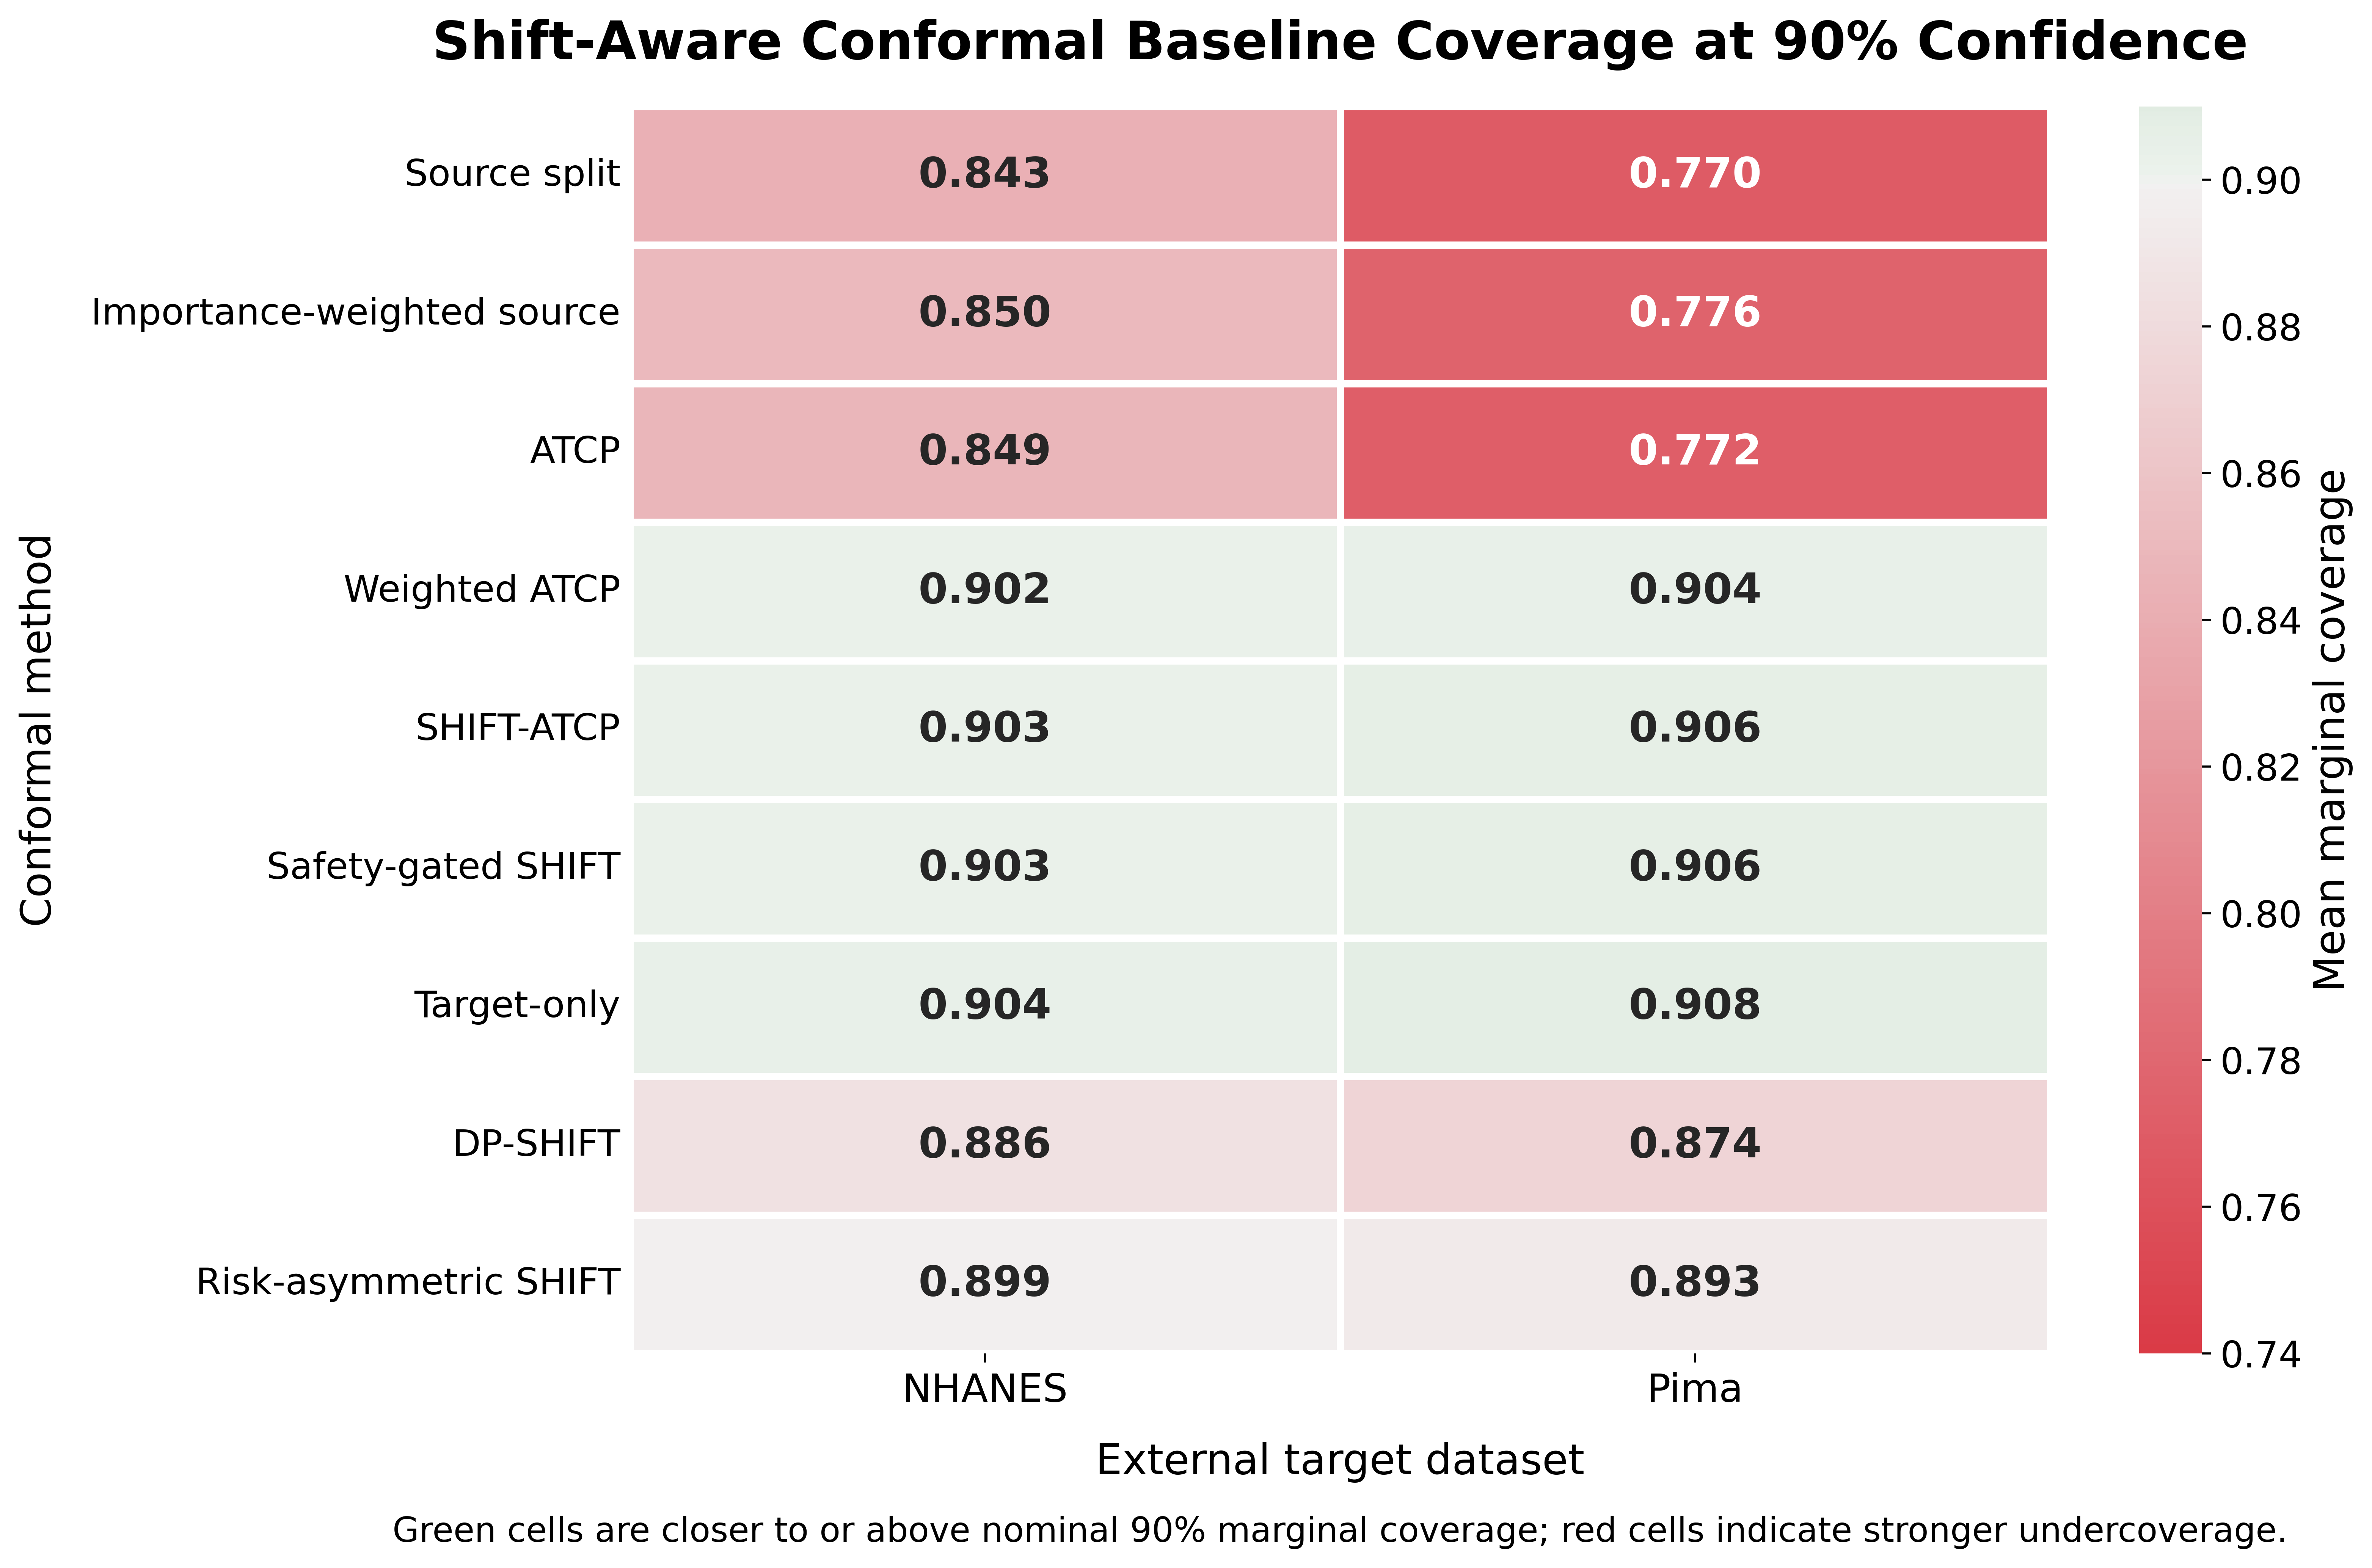
\includegraphics[width=0.95\textwidth]{figures/figure_shift_aware_conformal_baselines.png}
\caption{Shift-aware conformal baseline comparison at 90\% confidence. The plot compares source-only conformal prediction, importance-weighted conformal prediction, target-only conformal prediction, conventional ATCP, weighted ATCP, SHIFT-ATCP, and clinically protected variants.}
\label{fig:shift_baselines_insert}
\end{figure*}

\begin{figure*}[!t]
\centering
\includegraphics[width=0.95\textwidth]{figures/figure_clinical_reliability_tradeoff_shift_atcp_variants.png}
\caption{Clinical Reliability Trade-off of SHIFT-ATCP Variants. The figure separates marginal coverage, diabetes-positive coverage, average set size, and clinical cost for NHANES and Pima.}
\label{fig:clinical_tradeoff_insert}
\end{figure*}

\begin{figure*}[!t]
\centering
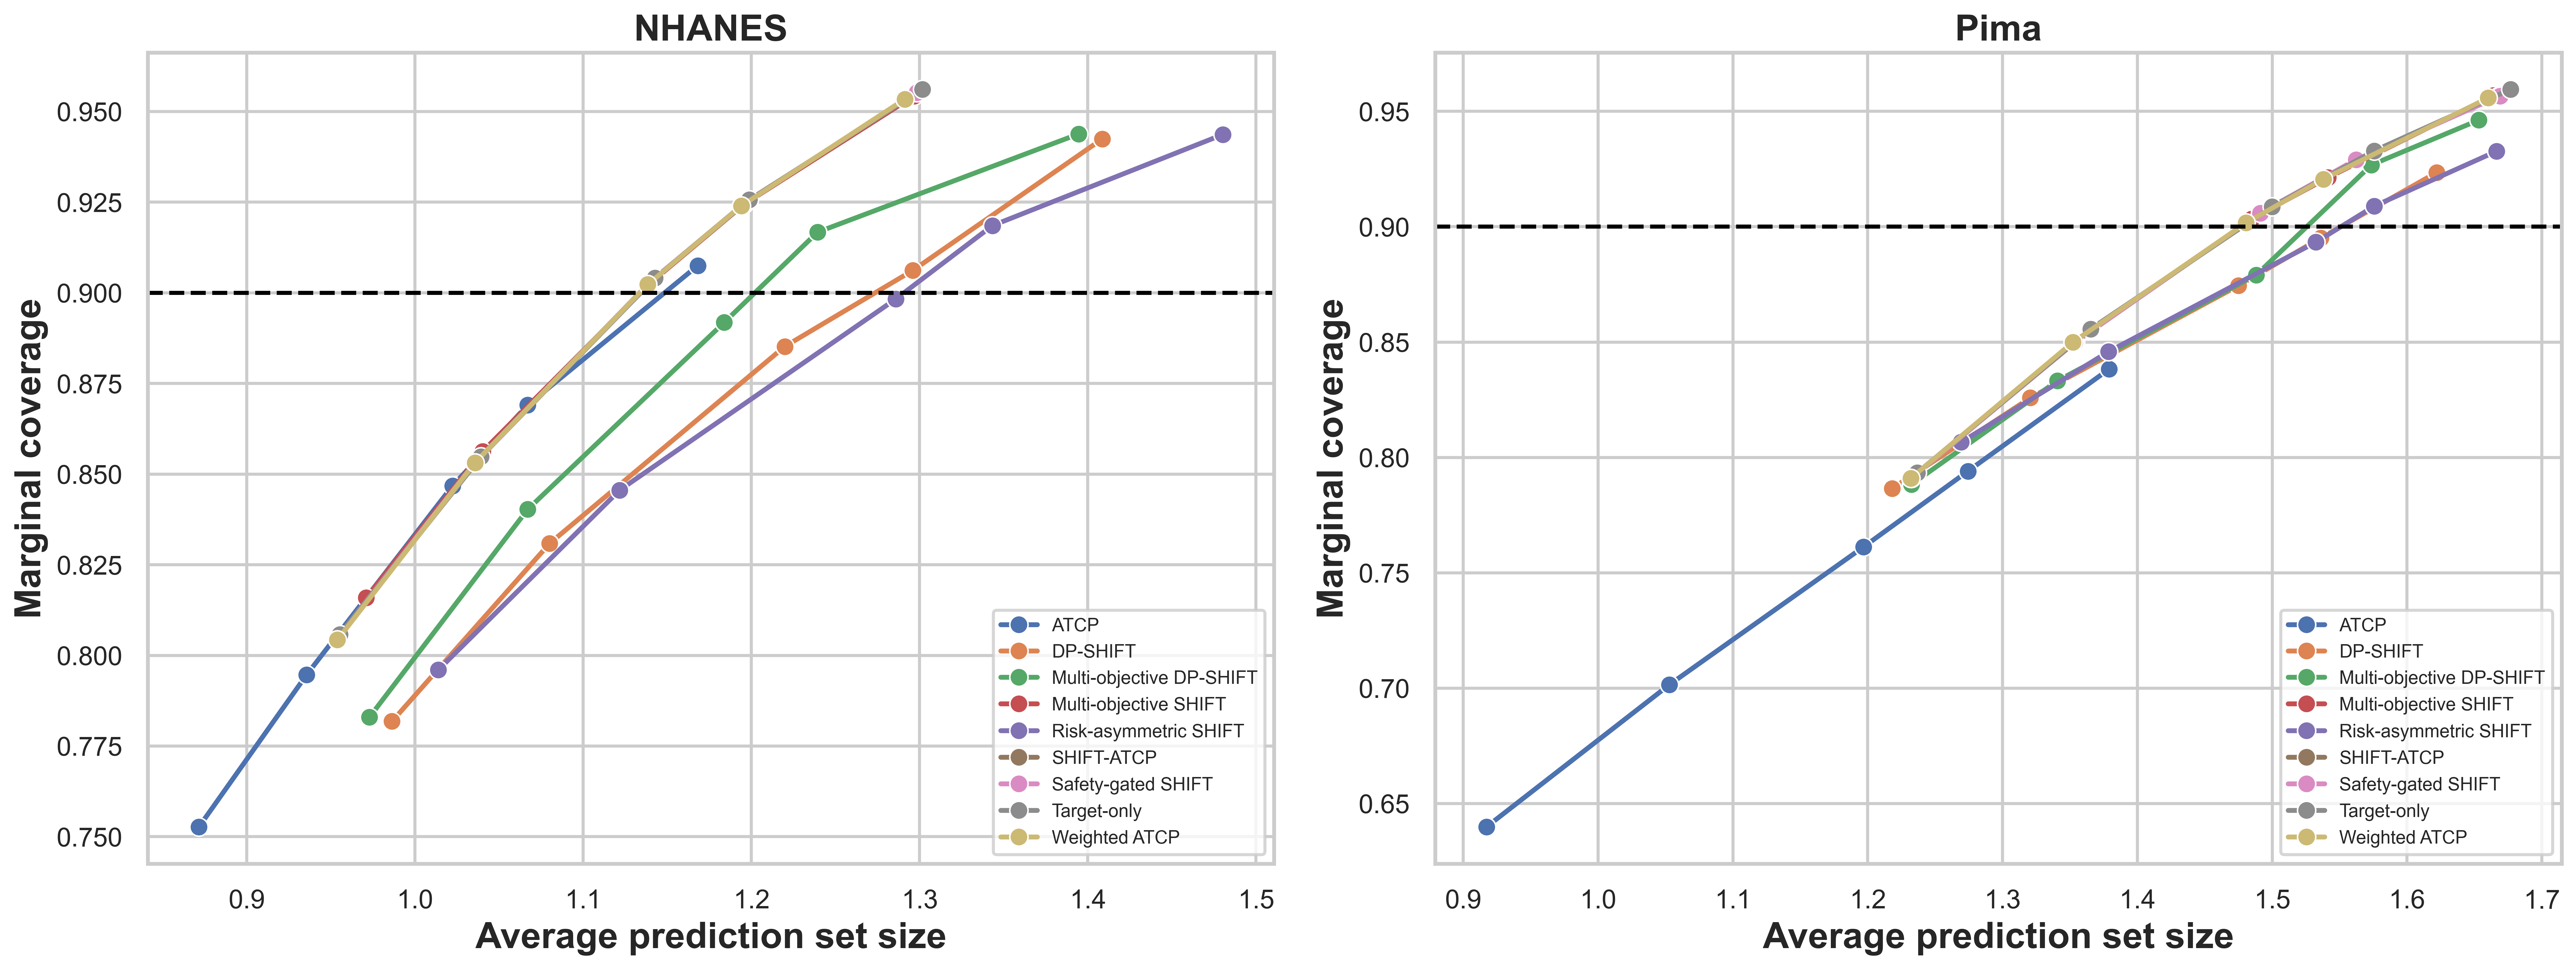
\includegraphics[width=0.95\textwidth]{figures/figure_shift_atcp_coverage_efficiency_frontier.png}
\caption{Coverage-efficiency frontier for SHIFT-ATCP variants across confidence levels. The frontier shows the trade-off between higher coverage and larger prediction sets or referral burden.}
\label{fig:coverage_frontier_insert}
\end{figure*}

\begin{figure*}[!t]
\centering
\includegraphics[width=0.95\textwidth]{figures/figure_shift_atcp_clinical_referral_cost.png}
\caption{Clinical referral and cost profile for SHIFT-ATCP variants. Diabetes-protected methods increase referral and set size when needed, but reduce diabetes-positive undercoverage and clinical cost in the external target cohorts.}
\label{fig:clinical_referral_cost_insert}
\end{figure*}

\begin{figure*}[!t]
\centering
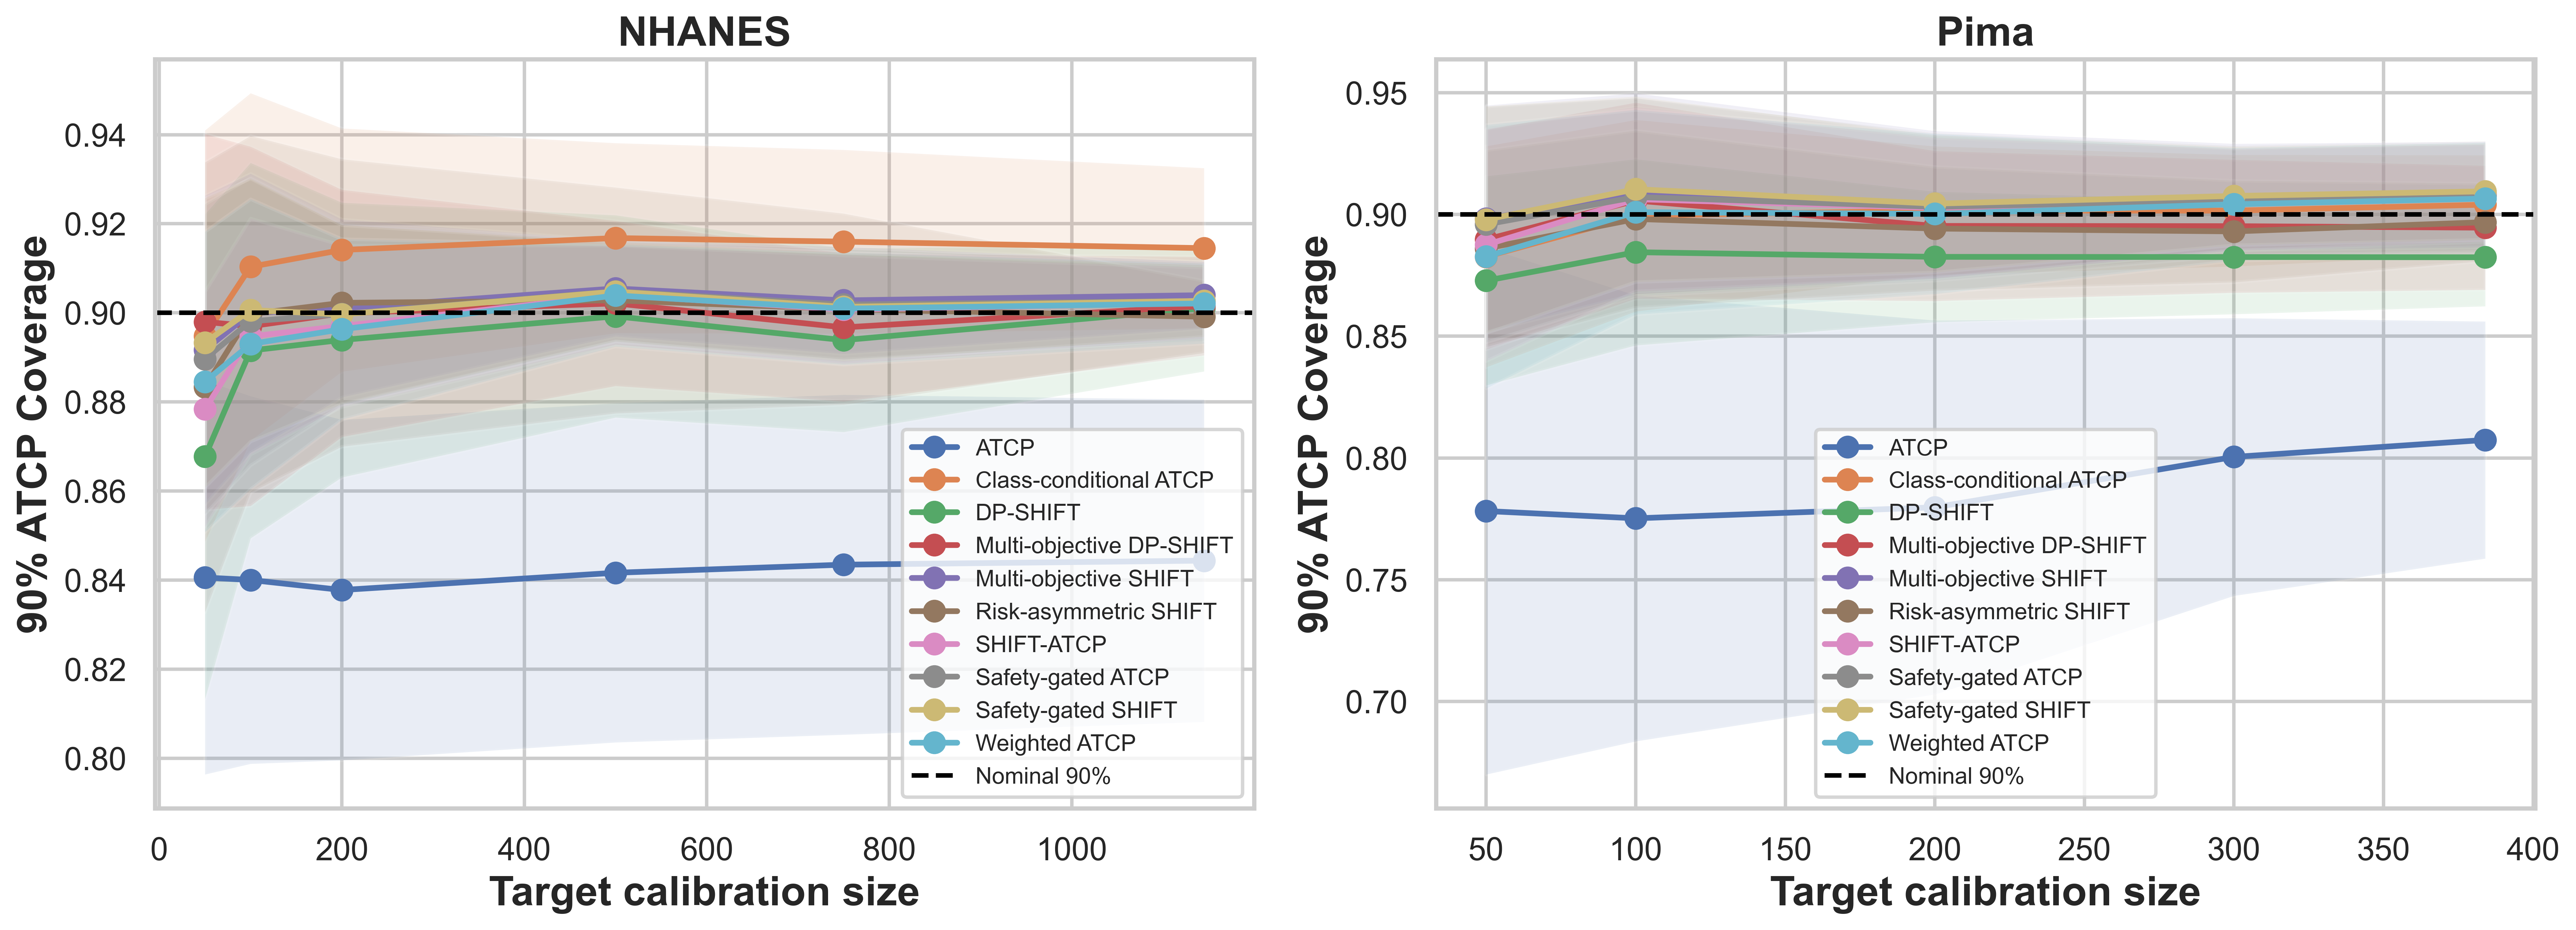
\includegraphics[width=0.95\textwidth]{figures/figure_target_calibration_size_ablation_coverage.png}
\caption{Target calibration-size ablation for conformal coverage.}
\label{fig:ablation_coverage_insert}
\end{figure*}

\begin{figure*}[!t]
\centering
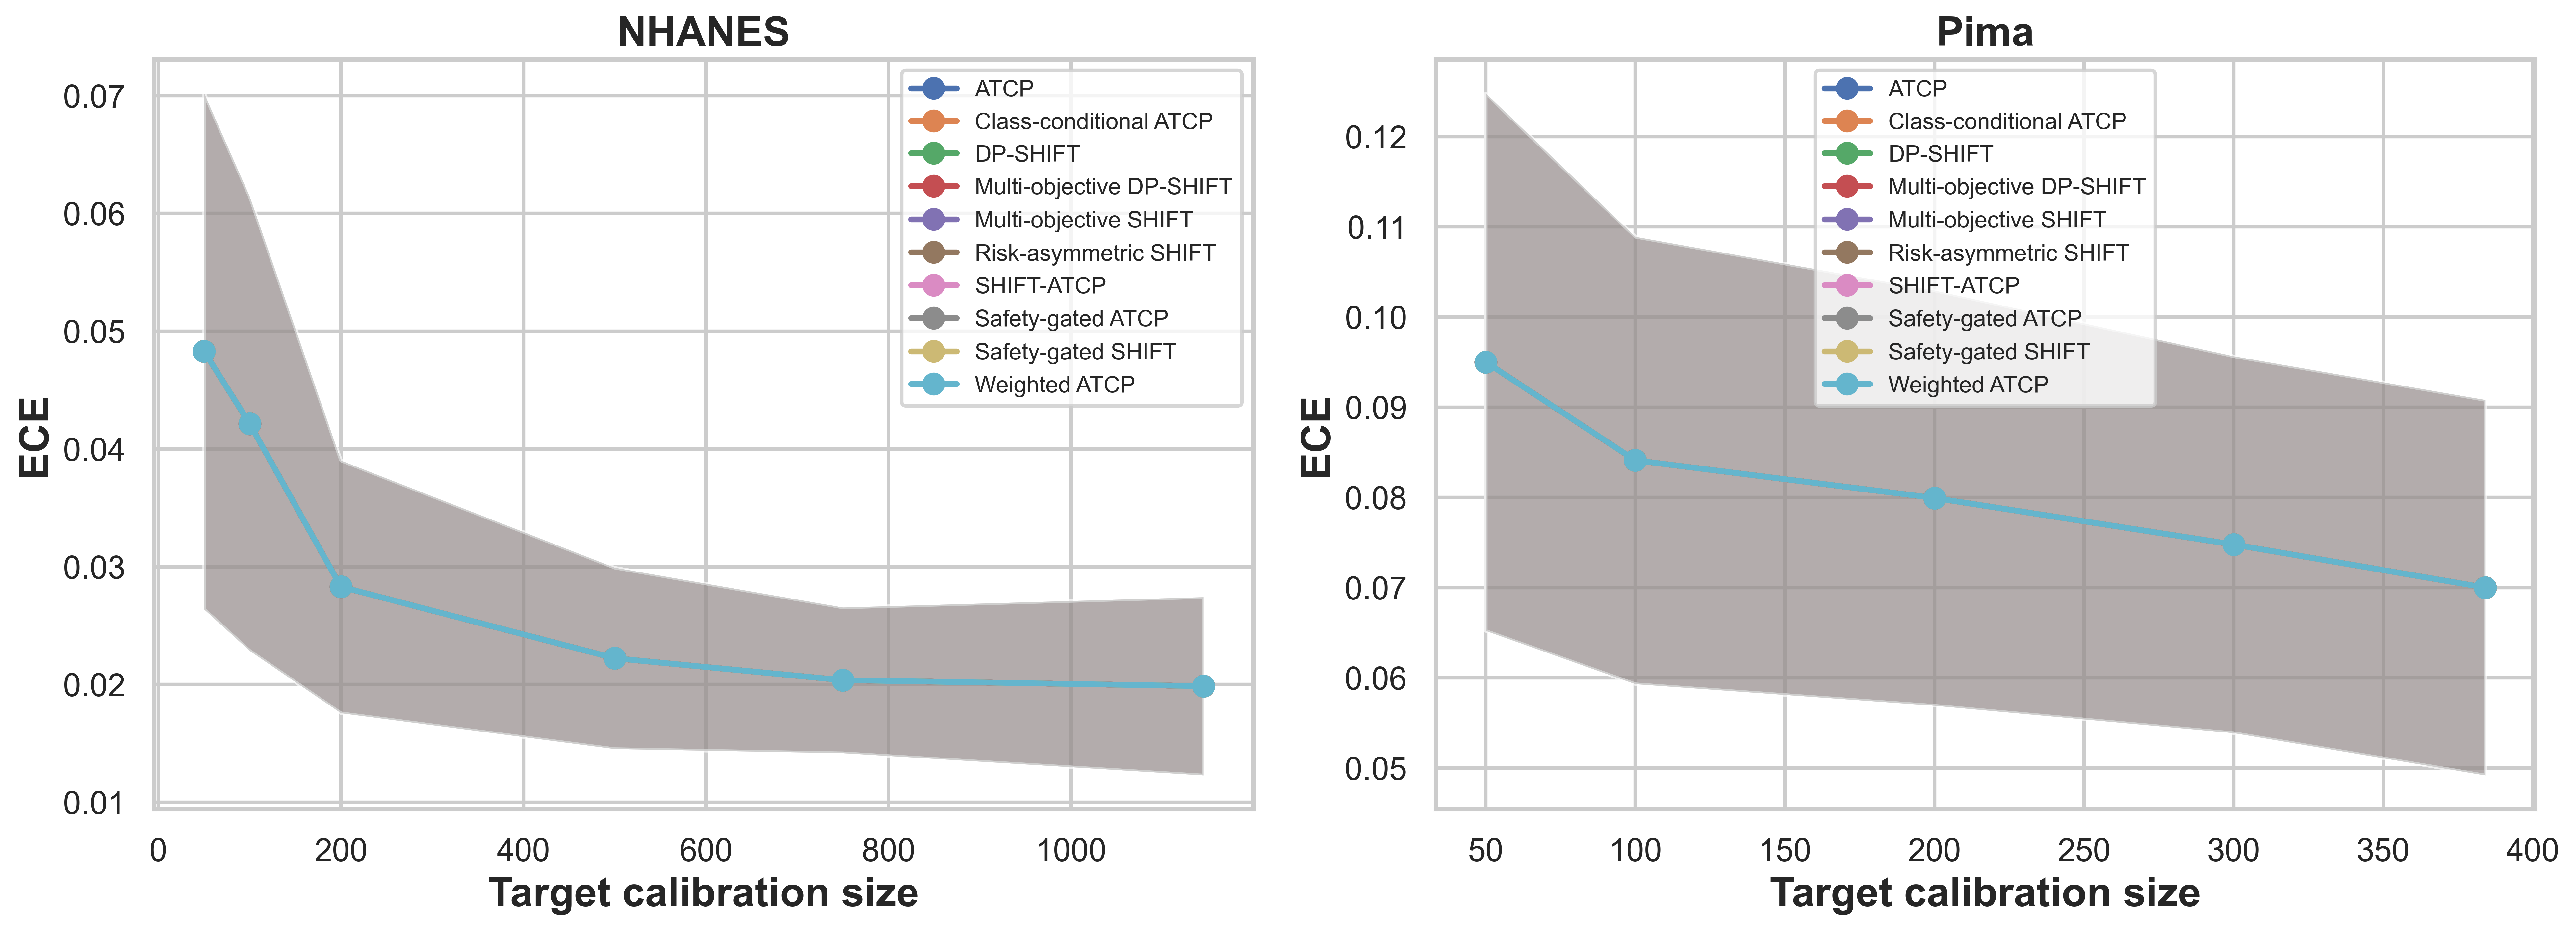
\includegraphics[width=0.95\textwidth]{figures/figure_target_calibration_size_ablation_ece.png}
\caption{Target calibration-size ablation for expected calibration error. The plot shows how probability calibration stability changes as the number of labeled target calibration samples increases.}
\label{fig:ablation_ece_insert}
\end{figure*}

\section{What to Remove or Replace From the Old Manuscript}
\begin{enumerate}
    \item Remove or comment the Helvetica font override:
    \texttt{\textbackslash usepackage[scaled]\{helvet\}} and
    \texttt{\textbackslash renewcommand\{\textbackslash familydefault\}\{\textbackslash sfdefault\}}.
    \item Replace the long title with the cleaner title in this file.
    \item Replace the long abstract with the shorter abstract in this file.
    \item Replace the old contribution list with the revised five-point list.
    \item Replace any unclear ECE explanation with the split-specific ECE table and text in this file.
    \item Replace the old clinical trade-off table with the updated version that includes target-only conformal.
    \item Do not make weighted ATCP the main story. In the main text, emphasize old ATCP, safety-gated SHIFT-ATCP, DP-SHIFT-ATCP, and risk-asymmetric SHIFT as sensitivity analysis.
    \item Remove any language that implies source calibration directly improved the final target threshold under severe shift. Use the discussion paragraph explaining automatic source rejection.
    \item Replace vague clinical-cost text with the exact cost formula and cost values from this file.
    \item Replace vague DP-SHIFT selection text with the exact score formula and fixed score weights from this file.
    \item In the ablation section, replace ``repeated stratified subsampling'' with ``20 repeated stratified subsamples.''
    \item Check the repository spelling in Code Availability. If the repository is truly named \texttt{Confirmal\_Prediction}, keep it; otherwise correct it to \texttt{Conformal\_Prediction}.
\end{enumerate}

\section{Reference Keys to Check in ref.bib}
Before compiling the final manuscript, confirm that the following citation keys exist:
\begin{verbatim}
who2023diabetes
datasetShift
plattScaling
zadrozny2002
guo2017
kull2017
vovk2005
shafer2008
angelopoulos2023
tripod
randomforest
xgboost
lightgbm
catboost
mustafa2023dataset
nhanes2018overview
smith1988using
\end{verbatim}

\end{document}
